% OpenAI Math Digest; follows the existing Schnell diagram style.
\documentclass[border=12pt]{standalone}
\def\pgfsysdriver{pgfsys-dvisvgm.def}
\usepackage[dvisvgm]{xcolor}
\usepackage{xeCJK}
\setCJKmainfont{HaranoAjiGothic-Regular.otf}[BoldFont=HaranoAjiGothic-Bold.otf]
\setCJKsansfont{HaranoAjiGothic-Regular.otf}[BoldFont=HaranoAjiGothic-Bold.otf]
\usepackage{amsmath,amssymb,tikz,lmodern}
\usetikzlibrary{arrows.meta,positioning,calc}
\renewcommand{\familydefault}{\sfdefault}
\definecolor{ink}{HTML}{25322F}
\definecolor{green}{HTML}{246657}
\definecolor{tint}{HTML}{EEF4F0}
\definecolor{soft}{HTML}{C6D2CC}
\definecolor{muted}{HTML}{52615B}
\definecolor{amber}{HTML}{866321}
\newif\ifJapanese
\newcommand{\Tx}[2]{\ifJapanese #1\else #2\fi}
\newcommand{\heading}[2]{{\color{green}\bfseries\Tx{#1}{#2}}\\[5pt]}
\newcommand{\refurl}[2]{\special{dvisvgm:raw <a xlink:href="#1" target="_blank" rel="noopener noreferrer">}{\color{green}\underline{\strut #2}}\special{dvisvgm:raw </a>}}
\newcommand{\R}[2]{\expandafter\refurl\expandafter{\csname source#1\endcsname}{#2}}
\tikzset{
 card/.style={draw=soft,fill=white,rounded corners=2pt,align=left,text=ink,font=\fontsize{10.5}{14}\selectfont,inner xsep=12pt,inner ysep=10pt,text width=14.4cm},
 result/.style={card,draw=green,fill=tint,line width=.9pt},
 reason/.style={align=left,text=muted,font=\fontsize{9}{12}\selectfont,inner sep=0pt,text width=12.65cm},
 edge/.style={-{Stealth[length=2.4mm]},draw=green,line width=1pt},
}
\newcommand{\flow}[3]{
 \coordinate (#2-from) at ($(#1.south)+(-6.9,0)$);
 \coordinate (#2-to) at ($(#2.north)+(-6.9,0)$);
 \draw[edge] (#2-from)--(#2-to);
 \node[reason,anchor=west] at ($(#2-from)!.5!(#2-to)+(.55,0)$) {#3};
}

\expandafter\def\csname sourceOI\endcsname{https://github.com/openai/math/blob/fd4aeeb2ee4fc729c18d98444fed42fd0529eeeb/preprints/Orbifold-and-logarithmic-Iitaka-subadditivity-September-26-2026/paper.pdf}
\expandafter\def\csname sourceWV\endcsname{https://github.com/openai/math/blob/fd4aeeb2ee4fc729c18d98444fed42fd0529eeeb/preprints/Logarithmic-Kodaira-dimension-and-whole-fiber-variation-September-26-2026/paper.pdf}
\expandafter\def\csname sourceRA\endcsname{https://github.com/openai/math/blob/fd4aeeb2ee4fc729c18d98444fed42fd0529eeeb/preprints/The-reverse-logarithmic-Kodaira-inequality-and-additivity-September-26-2026/paper.pdf}
\expandafter\def\csname sourcePH\endcsname{https://github.com/openai/math/blob/fd4aeeb2ee4fc729c18d98444fed42fd0529eeeb/preprints/Projective-Hodge-lines-and-ordinary-Iitaka-subadditivity-September-27-2026/paper.pdf}
\expandafter\def\csname sourceBS\endcsname{https://github.com/openai/math/blob/fd4aeeb2ee4fc729c18d98444fed42fd0529eeeb/preprints/B-semiampleness-for-compact-log-smooth-Kahler-fibrations-September-10-2026/paper.pdf}
\expandafter\def\csname sourceLA\endcsname{https://github.com/openai/math/blob/adc7f1241b42e322a6451854ab7e4b4c146bf78a/preprints/Log-abundance-in-characteristic-zero-September-24-2026/paper.pdf}
\expandafter\def\csname sourceKA\endcsname{https://github.com/openai/math/blob/adc7f1241b42e322a6451854ab7e4b4c146bf78a/preprints/Log-abundance-for-compact-Kahler-spaces-under-logarithmic-Iitaka-subadditivity-October-4-2026/main.pdf}
\expandafter\def\csname sourceCK\endcsname{https://github.com/openai/math/blob/adc7f1241b42e322a6451854ab7e4b4c146bf78a/preprints/Conditional-good-minimal-models-for-compact-Kahler-fourfolds-October-5-2026/paper.pdf}
\expandafter\def\csname sourceOV\endcsname{https://github.com/openai/math/blob/fd4aeeb2ee4fc729c18d98444fed42fd0529eeeb/overview.pdf}
\expandafter\def\csname sourceCONTENTS\endcsname{https://github.com/openai/math/blob/fd4aeeb2ee4fc729c18d98444fed42fd0529eeeb/CONTENTS.md}
\Japanesefalse
\begin{document}
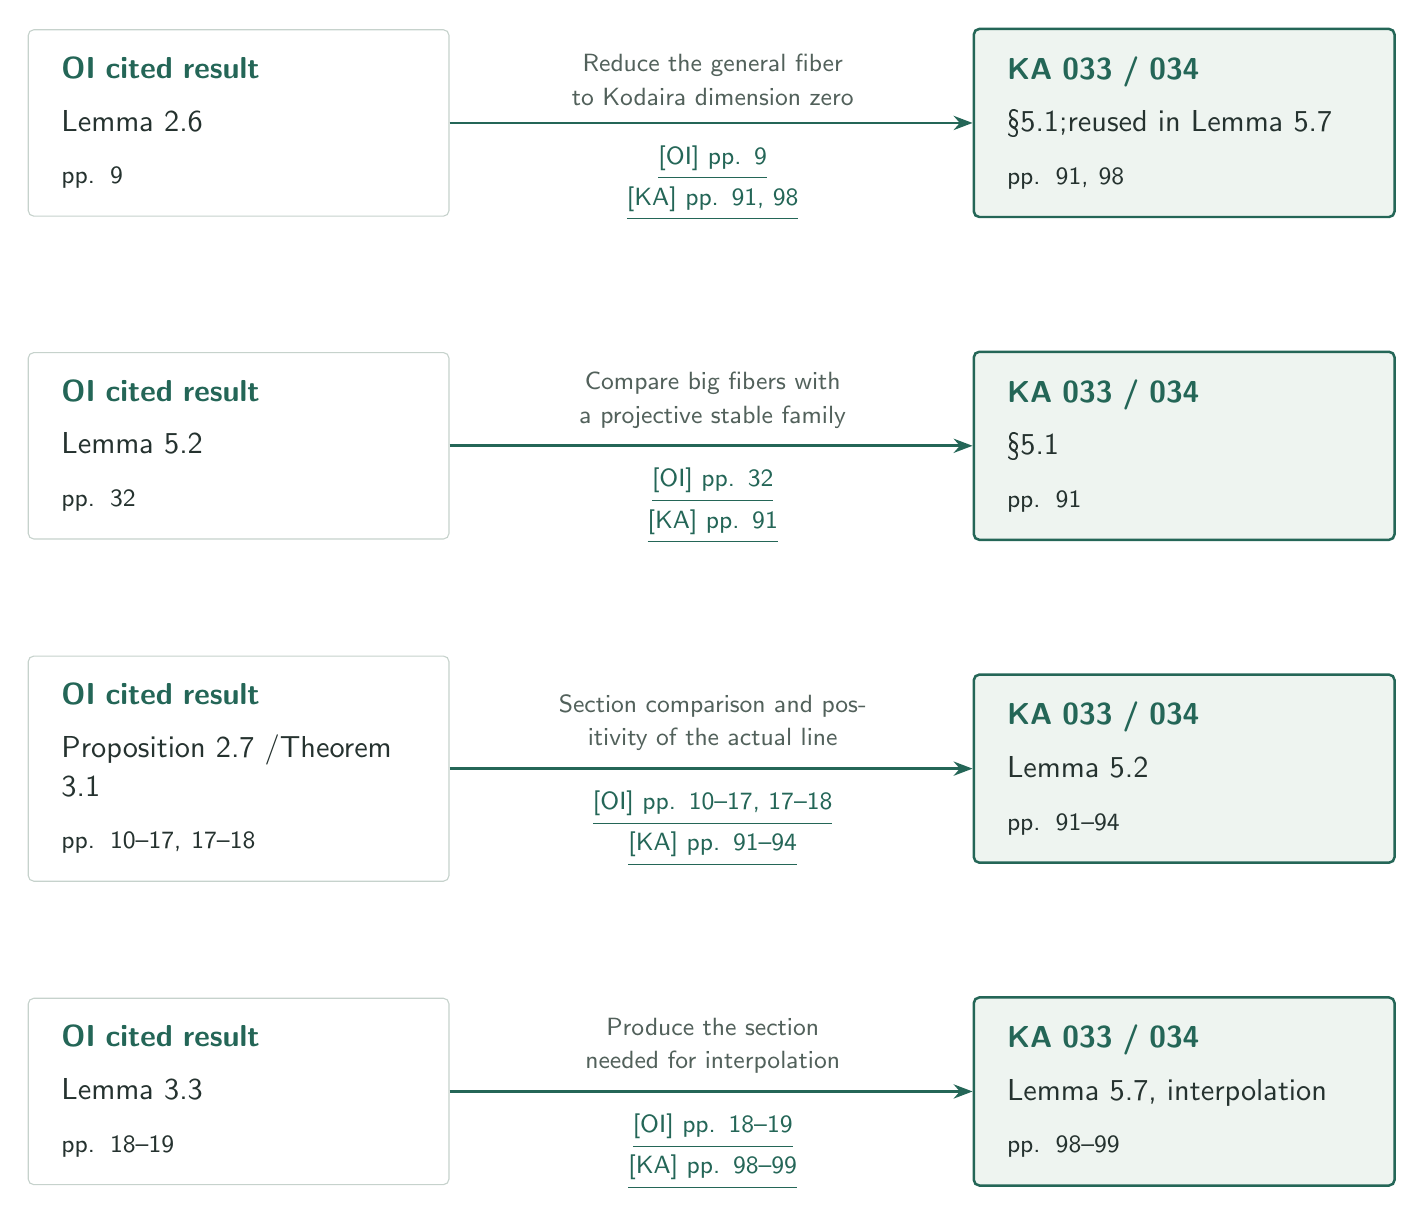
\begin{tikzpicture}
\node[card,text width=4.5cm,minimum height=2.3cm,anchor=west] (s0) at (0,0.0) {\heading{OI 引用する結果}{OI cited result}Lemma 2.6\\[5pt]{\small pp. 9}};
\node[result,text width=4.5cm,minimum height=2.3cm,anchor=west] (t0) at (12.0,0.0) {\heading{KA 034との接続}{KA 033 / 034}\S 5.1;\allowbreak \Tx{再使用：}{reused in} Lemma 5.7\\[5pt]{\small pp. 91, 98}};
\draw[edge] (s0.east)--(t0.west);
\node[reason,text width=5.1cm,align=center,anchor=south] at (8.7,0.22) {\Tx{一般ファイバーを小平次元0へ}{Reduce the general fiber to Kodaira dimension zero}};
\node[reason,text width=5.1cm,align=center,anchor=north] at (8.7,-0.22) {\R{OI}{[OI] pp. 9}\\\R{KA}{[KA] pp. 91, 98}};
\node[card,text width=4.5cm,minimum height=2.3cm,anchor=west] (s1) at (0,-4.1) {\heading{OI 引用する結果}{OI cited result}Lemma 5.2\\[5pt]{\small pp. 32}};
\node[result,text width=4.5cm,minimum height=2.3cm,anchor=west] (t1) at (12.0,-4.1) {\heading{KA 034との接続}{KA 033 / 034}\S 5.1\\[5pt]{\small pp. 91}};
\draw[edge] (s1.east)--(t1.west);
\node[reason,text width=5.1cm,align=center,anchor=south] at (8.7,-3.8799999999999994) {\Tx{bigなファイバーを射影的stable familyへ}{Compare big fibers with a projective stable family}};
\node[reason,text width=5.1cm,align=center,anchor=north] at (8.7,-4.319999999999999) {\R{OI}{[OI] pp. 32}\\\R{KA}{[KA] pp. 91}};
\node[card,text width=4.5cm,minimum height=2.3cm,anchor=west] (s2) at (0,-8.2) {\heading{OI 引用する結果}{OI cited result}Proposition 2.7 /\allowbreak Theorem 3.1\\[5pt]{\small pp. 10--17, 17--18}};
\node[result,text width=4.5cm,minimum height=2.3cm,anchor=west] (t2) at (12.0,-8.2) {\heading{KA 034との接続}{KA 033 / 034}Lemma 5.2\\[5pt]{\small pp. 91--94}};
\draw[edge] (s2.east)--(t2.west);
\node[reason,text width=5.1cm,align=center,anchor=south] at (8.7,-7.9799999999999995) {\Tx{切断比較と実際のHodge lineの正値性}{Section comparison and positivity of the actual line}};
\node[reason,text width=5.1cm,align=center,anchor=north] at (8.7,-8.42) {\R{OI}{[OI] pp. 10--17, 17--18}\\\R{KA}{[KA] pp. 91--94}};
\node[card,text width=4.5cm,minimum height=2.3cm,anchor=west] (s3) at (0,-12.299999999999999) {\heading{OI 引用する結果}{OI cited result}Lemma 3.3\\[5pt]{\small pp. 18--19}};
\node[result,text width=4.5cm,minimum height=2.3cm,anchor=west] (t3) at (12.0,-12.299999999999999) {\heading{KA 034との接続}{KA 033 / 034}Lemma 5.7, \Tx{補間}{interpolation}\\[5pt]{\small pp. 98--99}};
\draw[edge] (s3.east)--(t3.west);
\node[reason,text width=5.1cm,align=center,anchor=south] at (8.7,-12.079999999999998) {\Tx{補間に使う非零切断を作る}{Produce the section needed for interpolation}};
\node[reason,text width=5.1cm,align=center,anchor=north] at (8.7,-12.52) {\R{OI}{[OI] pp. 18--19}\\\R{KA}{[KA] pp. 98--99}};
\end{tikzpicture}
\end{document}
